\documentclass[oneside, a5paper,10pt]{article}

%------------Служебная информация, не меняй----------
\usepackage[TS1,T2A]{fontenc}
\usepackage[utf8]{inputenc}
\usepackage[english,russian]{babel}
\usepackage{indentfirst} %отступ в начале параграфа
\usepackage{amsmath,amsthm,amssymb} %математические библиотеки
\usepackage{graphicx}%Вставка картинок правильная
\usepackage{float}%"Плавающие" картинки
\usepackage{wrapfig}%Обтекание фигур (таблиц, картинок и прочего)
\usepackage{fancyhdr} %Колонтитул
\usepackage{geometry}
\geometry{
    left=1.5cm,% 1.9
    top=1.5cm,% 1.5
    right=1.5cm,% 1.9
    bottom=1.5cm,% 1.5
    headsep=0.5cm,%
    footskip=0.5cm,%
    includehead,%
    includefoot}
\textwidth 110mm
\textheight 170mm
\linespread{1.0}
\setlength{\parskip}{3pt}
%-----------------------------------------------------

\begin{document}
%--------Колонтитул конференции - не менять------------
\pagestyle{fancy}
\fancyhead{}\fancyfoot{}
\fancyhead[C]{Мультидисциплинарная молодежная конференция Центрального университета «Научный телеграф»}
\cfoot{\thepage}
%------------------------------------------------------

%--------Название статьи, лишнюю строку удали----------
\centerline{\bf СРАВНЕНИЕ РАВНОМЕРНОГО И ПРИОРИТИЗИРОВАННОГО} %название статьи
\centerline{\bf EXPERIENCE REPLAY ПРИ ОБУЧЕНИИ DQN-АГЕНТА}
\centerline{\bf В ИГРЕ «УГОЛКИ»}

\smallskip %отступ
%--------Информация об авторах -----------------------
\centerline{\bf}
\centerline{\bf \ \ А.~А. Самойлов$^{1,*}$}
\smallskip
\centerline{$^{1}$ Центральный университет}
\centerline{$^{*}$\it email: samoilov@centraluniversity.ru}
%-------------------------------------------------------
\bigskip %отступ

%--------Аннотация в 3 предложения-----------------------
В работе сравниваются равномерная (Uniform Replay) и приоритизированная (PER) стратегии выборки из буфера воспроизведения при обучении DQN в игре «Уголки». Реализованы среда на доске~$8\times8$, агенты-базисы и воспроизводимый evaluation pipeline с bootstrap-оценкой доверительных интервалов по 1000~партиям на пару. Оба агента статистически значимо превосходят случайную игру; при этом Uniform Replay демонстрирует более высокий win~rate ($23{,}5\%$ против $17{,}4\%$ у PER, $p<0{,}05$).
\medskip

%--------Ключевые слова - не более 5-----------------------
\textit{Ключевые слова:} обучение с подкреплением, DQN, \foreignlanguage{english}{prioritized experience replay}, игровые агенты, \foreignlanguage{english}{self-play}.

\medskip %отступ

\textbf{Актуальность.} DQN~\cite{Mnih15} стабилизирует обучение за счёт \foreignlanguage{english}{experience replay}. Равномерная выборка не учитывает информативность переходов, тогда как PER~\cite{Schaul16} приоритизирует переходы с высокой TD-ошибкой, что теоретически ускоряет сходимость. Сравнение этих стратегий в настольных играх с дискретным замаскированным пространством действий остаётся практически неисследованным.

\textbf{Постановка задачи.} Среда~--- доска $8\times8$ c 9~фишками у каждого игрока; разрешены ортогональные ходы и прыжки, диагонали запрещены; цель~--- перенести фишки в противоположный угол. Исследуется влияние стратегии replay на качество выученной политики при фиксированном числе эпизодов self-play.

\textbf{Метод.} Состояние кодируется тензором~$3\times8\times8$; нелегальные действия маскируются. Сеть всегда наблюдает позицию с точки зрения текущего игрока~--- это обеспечивает инвариантность к смене сторон. При PER приоритет и вероятность выборки перехода~$i$:
\begin{equation}\label{Eq1}
    p_i = \bigl(|\delta_i|+\varepsilon\bigr)^{\alpha},\quad
    P(i) = \frac{p_i}{\sum\nolimits_{j} p_j},
\end{equation}
где $\delta_i$~--- TD-ошибка, $\varepsilon>0$, $\alpha=0{,}6$. IS-веса корректируют смещение с анилингом $\beta{:}\ 0{,}4{\to}1{,}0$~\cite{Schaul16}.

\textbf{Экспериментальный протокол.} По 1500~эпизодов self-play при 2~random seed; оба варианта используют общий warm-start от имитационного обучения. Оценка~--- 1000~партий на каждую пару (Uniform$\times$2~seed, PER$\times$2~seed против Random, Greedy, Heuristic). Доверительные интервалы win~rate~--- 95\% bootstrap (10\,000 ресэмплов по отдельным партиям); для проверки превосходства используется bootstrap-ДИ разности.

\begin{figure}[H]
    \center
    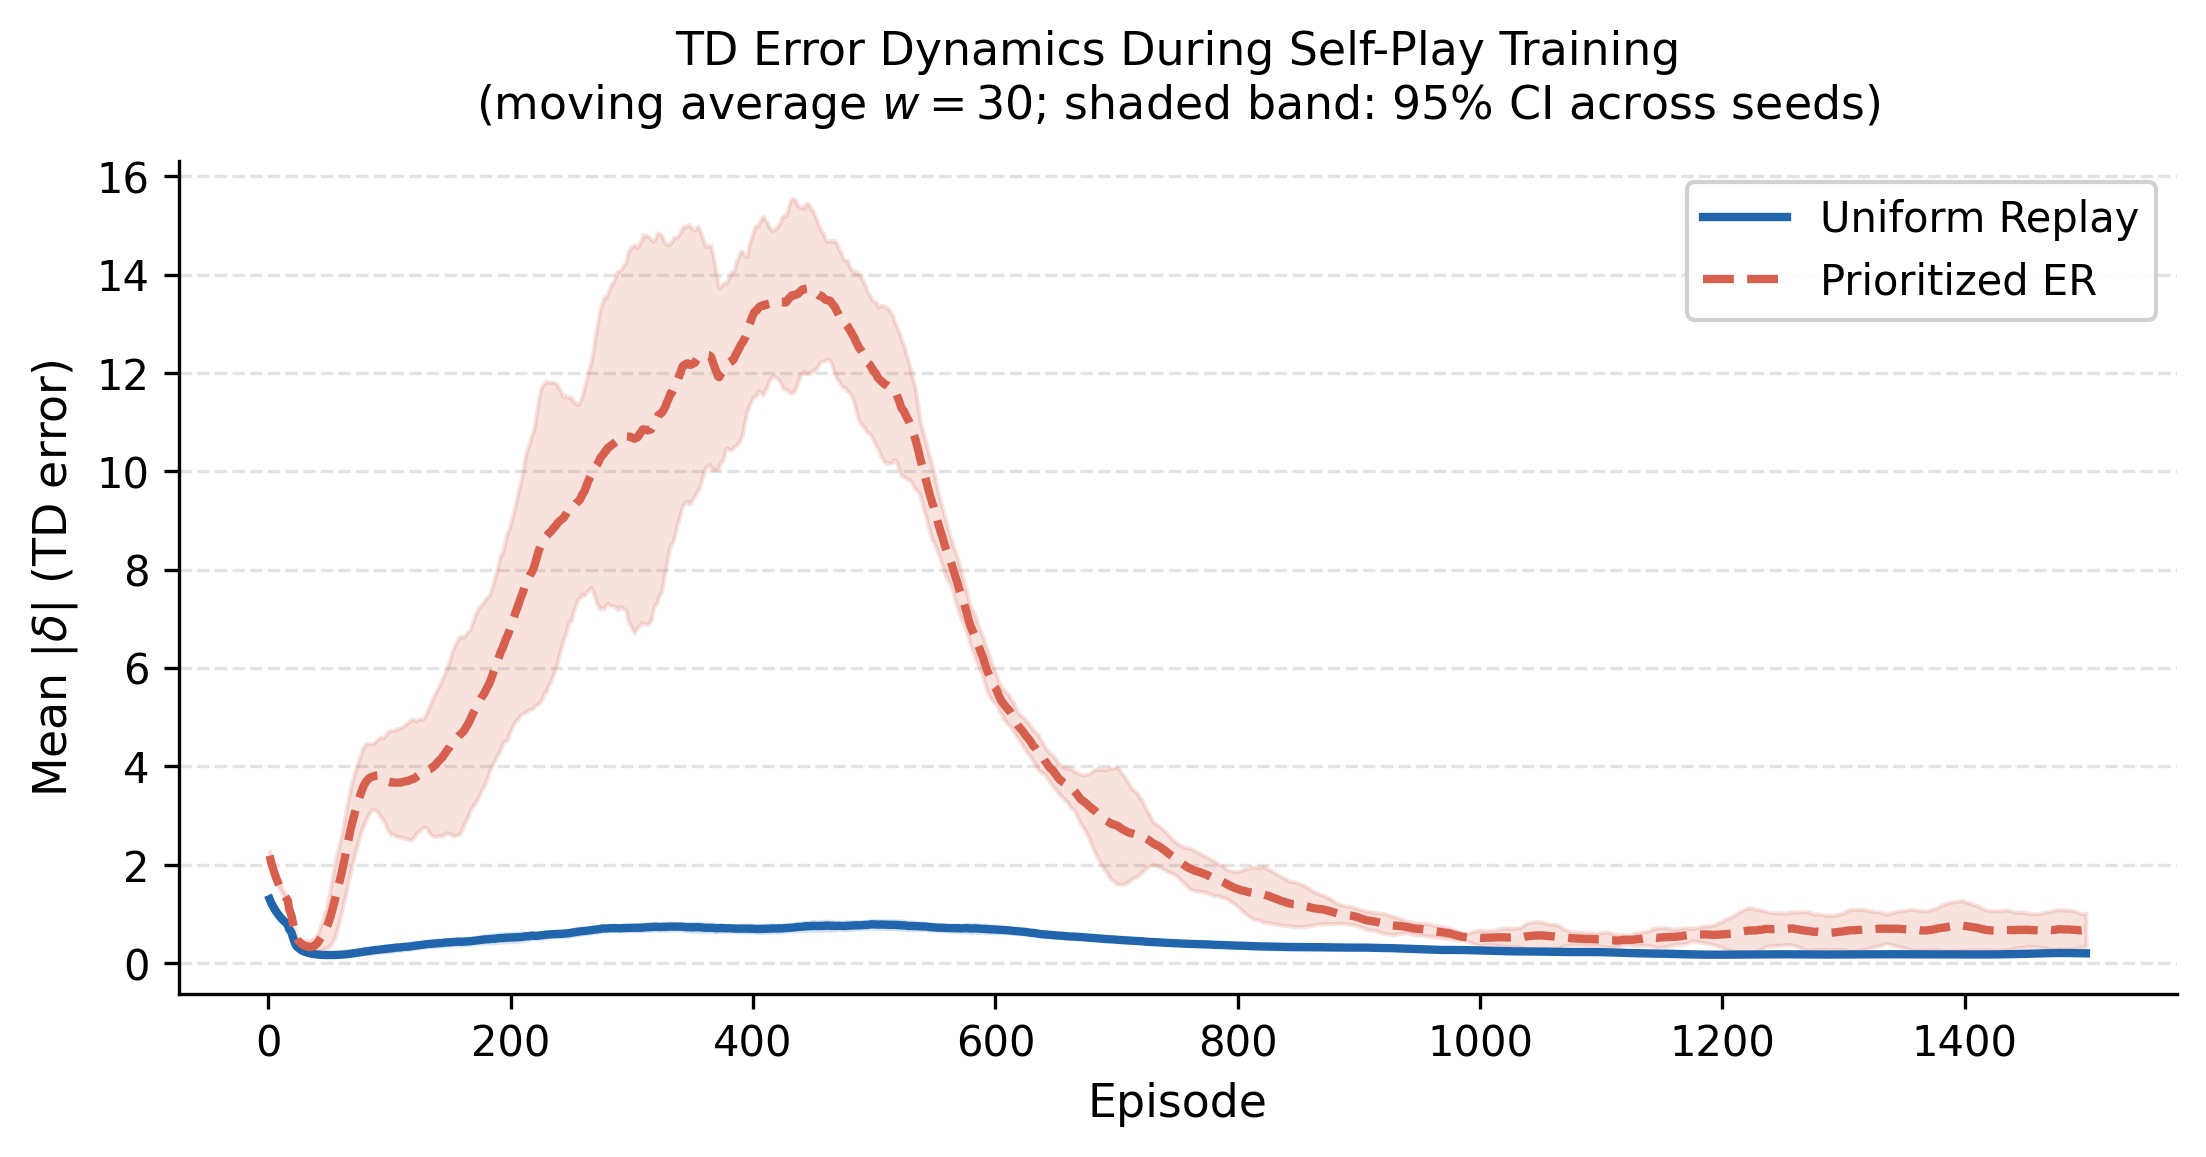
\includegraphics[width=0.93\linewidth]{figures/td_error_improved.png}
    \caption{Динамика средней абсолютной TD-ошибки~$|\delta|$ (скользящее среднее, $w{=}30$; полоса~--- 95\% CI по seed). PER демонстрирует характерный пик на ранних эпизодах.}
    \label{fig:td}
\end{figure}

\textbf{Результаты.} Рис.~\ref{fig:td} демонстрирует качественно различную динамику: при PER~$|\delta|$ резко возрастает в начале обучения (до~${\approx}12{,}7$), затем убывает~--- типичное поведение приоритизированной выборки, концентрирующей обновления на наиболее информативных переходах~\eqref{Eq1}. Uniform Replay даёт гладкое монотонное убывание~$|\delta|$.

\begin{figure}[H]
    \center
    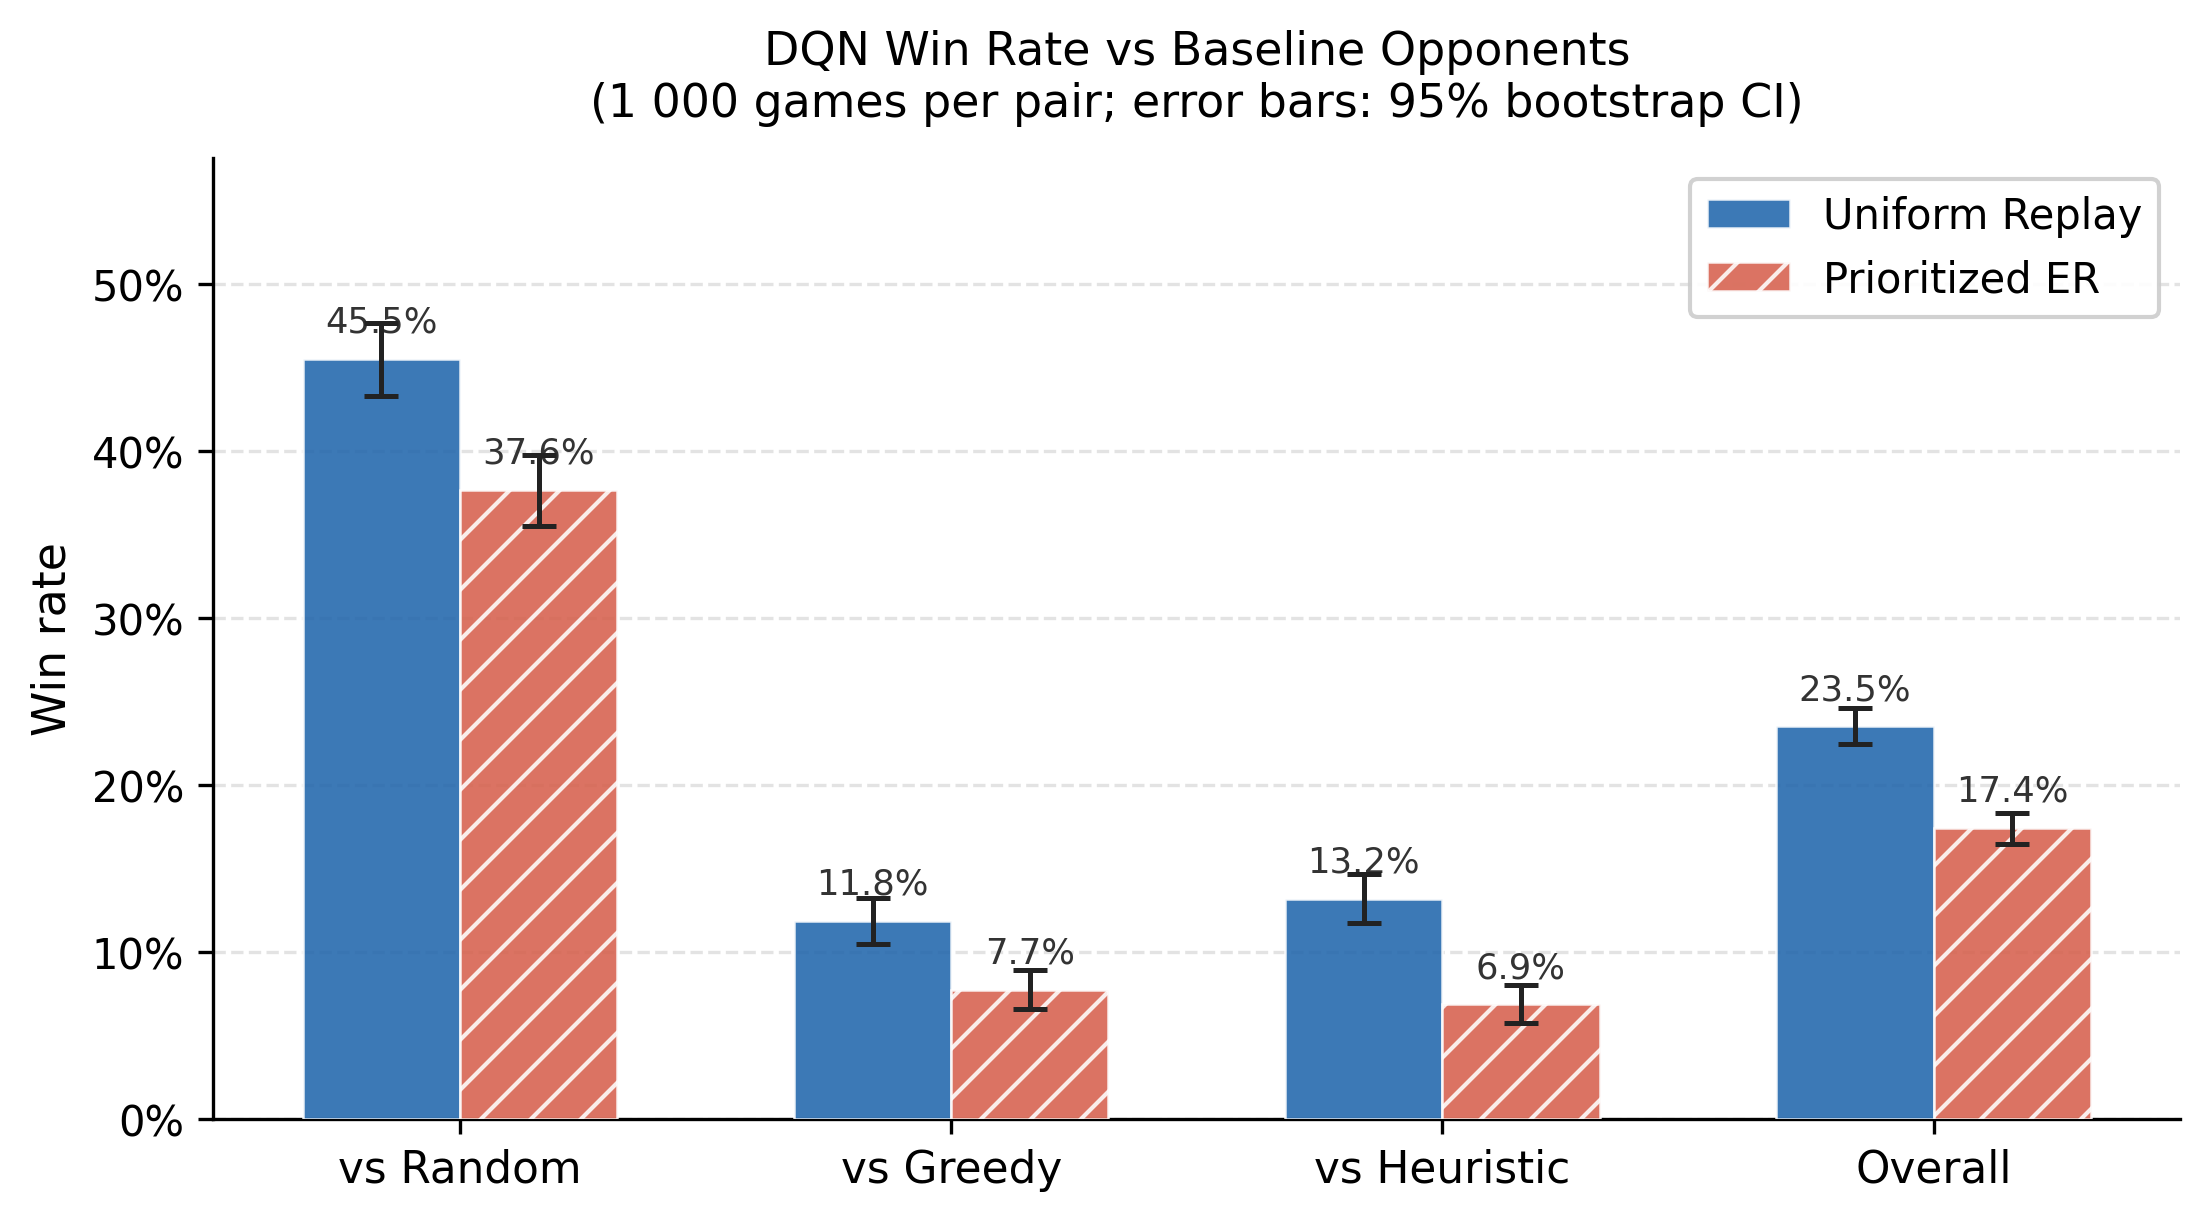
\includegraphics[width=0.93\linewidth]{figures/winrate_vs_opponents.png}
    \caption{Win~rate DQN-агентов против каждого соперника и суммарно (1000~партий на пару; планки~--- 95\% bootstrap CI).}
    \label{fig:wr}
\end{figure}

По итогам 6000~партий на каждую стратегию (рис.~\ref{fig:wr}) Uniform Replay достиг суммарного win~rate $23{,}5\%$ $[22{,}4\%;\,24{,}6\%]$, PER~--- $17{,}4\%$ $[16{,}4\%;\,18{,}3\%]$. Доверительные интервалы не пересекаются, а bootstrap-ДИ разности составляет $+6{,}1\%$ $[{+}4{,}6\%;\,{+}7{,}5\%]$: ноль не входит в интервал, что подтверждает статистическую значимость превосходства Uniform Replay в данных условиях. При этом оба агента конкурентоспособны против рукописных базисов (рис.~\ref{fig:random}).

\begin{figure}[H]
    \center
    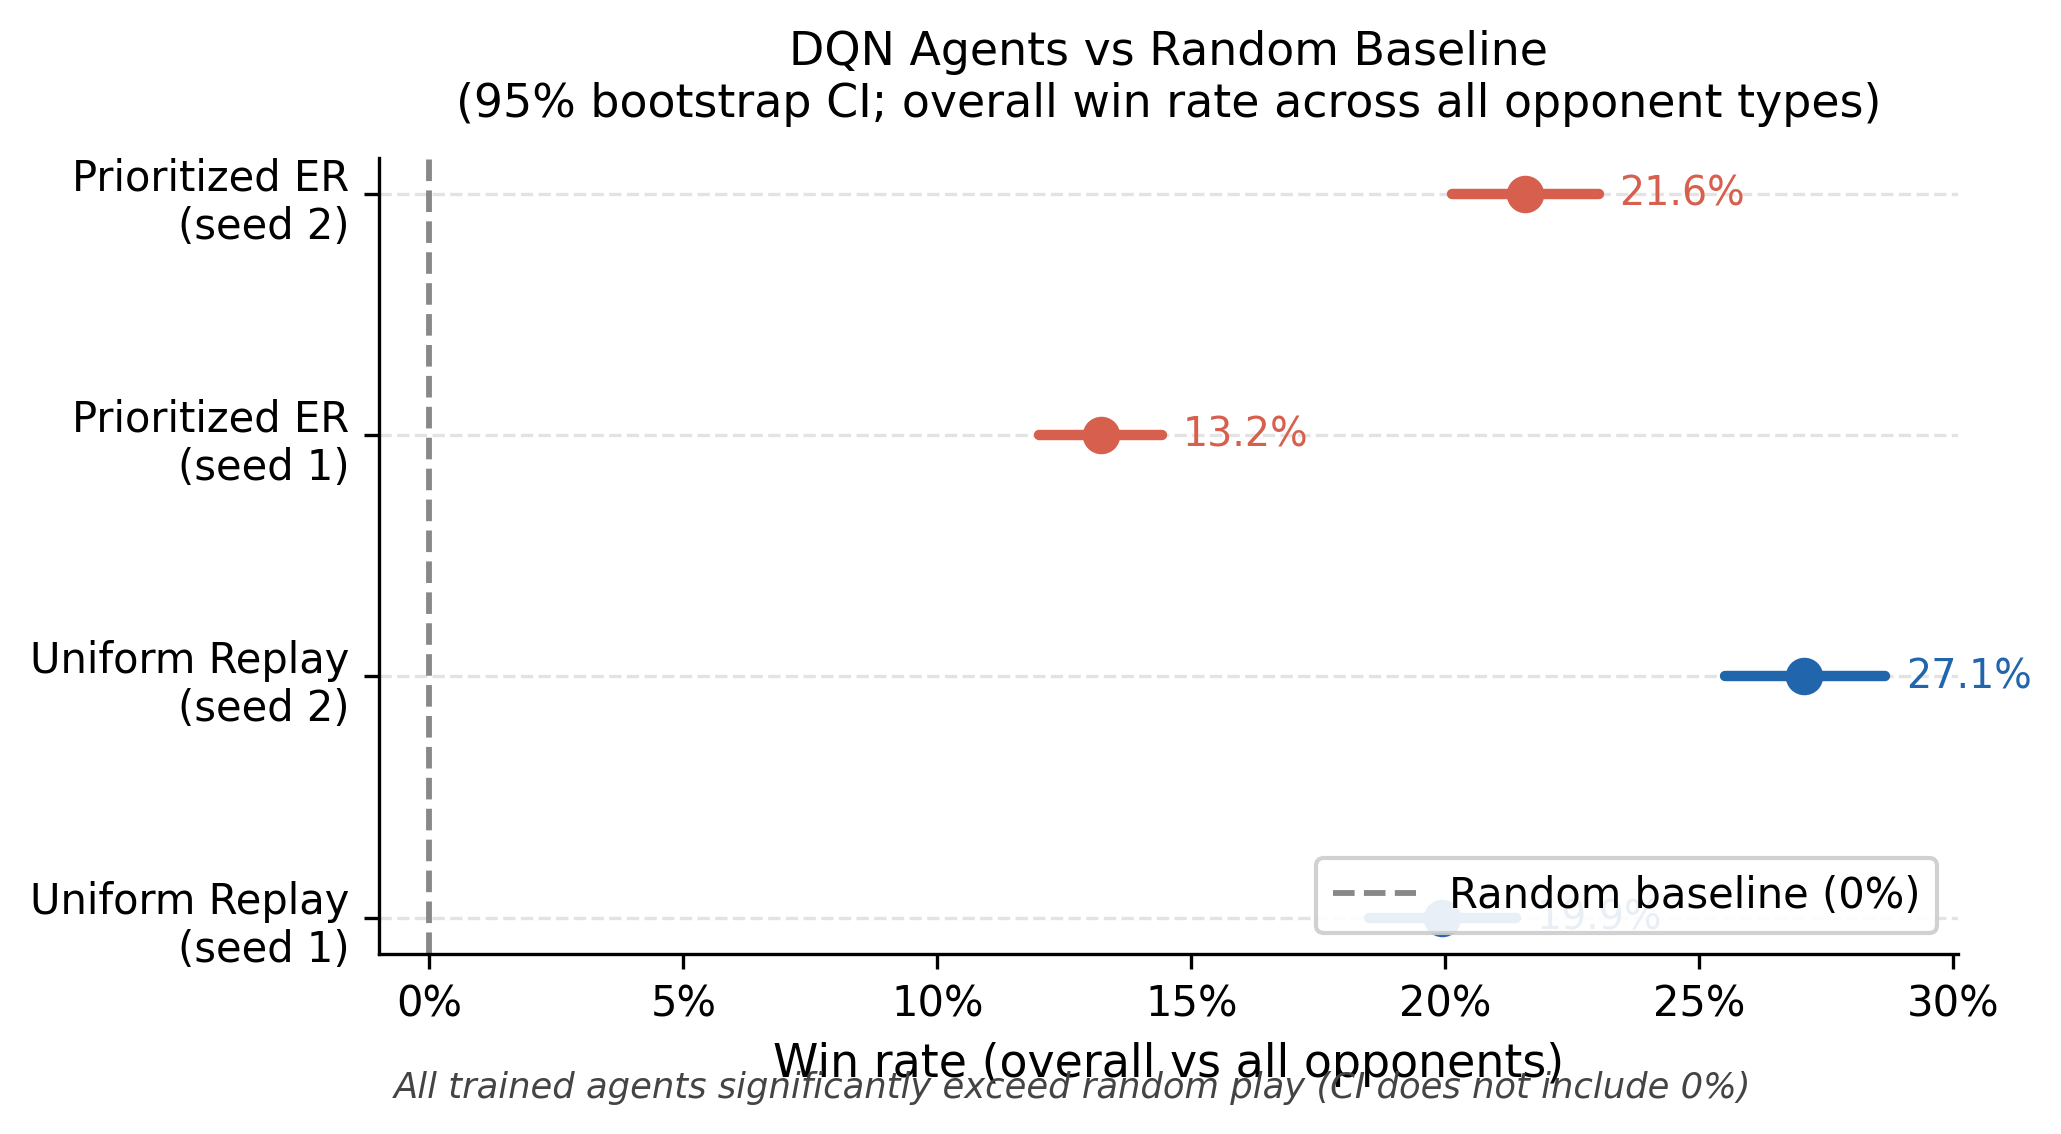
\includegraphics[width=0.93\linewidth]{figures/vs_random_baseline.png}
    \caption{Суммарный win~rate каждого DQN-агента (по всем типам соперников). Пунктир~--- уровень случайной игры. 95\% bootstrap CI.}
    \label{fig:random}
\end{figure}

Нижние границы 95\%~CI всех четырёх агентов ($12{,}0\%$ и выше) существенно превышают нулевой уровень случайной игры (рис.~\ref{fig:random}), то есть оба варианта DQN статистически значимо превосходят Random. В прямом матче лучший Uniform~(seed~2) выиграл у лучшего PER~(seed~2) на 1000~партиях.

\textbf{Заключение.} Реализованы среда «Уголки» для RL, агенты-базисы и воспроизводимый evaluation pipeline с bootstrap-статистикой. Оба обученных DQN-агента статистически значимо превосходят случайную игру и демонстрируют конкурентный уровень против рукописных стратегий. Uniform Replay показал значимо более высокий win~rate при 1500~эпизодах self-play ($+6{,}1\%$, ДИ разности не содержит нуль), что согласуется с известной чувствительностью PER к настройке гиперпараметров~\cite{Hessel18}. Проверка гипотезы о превосходстве PER в режиме большего числа эпизодов остаётся перспективой будущих исследований.

\begin{thebibliography}{00}

\setlength{\itemsep}{1.0pt plus 1.0pt}

\bibitem{Mnih15}
\textit{Mnih V. et al.} Human-level control through deep reinforcement learning // Nature.~--- 2015.~--- Vol.~518.~--- P.~529--533.

\bibitem{Schaul16}
\textit{Schaul T., Quan J., Antonoglou I., Silver D.} Prioritized Experience Replay // ICLR.~--- 2016.

\bibitem{Hessel18}
\textit{Hessel M. et al.} Rainbow: Combining Improvements in Deep Reinforcement Learning // AAAI.~--- 2018.~--- P.~3215--3222.

\end{thebibliography}

\end{document}
